\documentclass[10pt]{article}
\usepackage[margin=1in]{geometry}
\usepackage{multicol}
%\usepackage{setspace}
%\usepackage{amstext}
%\usepackage{amsmath}
%\usepackage{enumerate}
\usepackage{graphicx}
\usepackage{wrapfig}

\title{
	\textbf{
		Creating a Turn-Based Conflict Resolution Simulator
	}
}
\author{Noah Zimmt and Dakota Szabo}
\date{May 8, 2012}

\begin{document}
	\maketitle
	\begin{abstract}
		In this paper, we describe a territory-conquest simulation modeled on the classic board game \emph{RISK} and present a parallelized method for efficiently simulating multiple rounds of the model. 
		Players compete on a gameboard represented by an undirected graph, with vertices and edges representing territories and their borders, respectively. 
		Using MPI, we distributed the computation and resolution of player actions between multiple compute nodes in order to acheive the speed neccessary to simulate massive games in a reasonable amount of time. 
		This was acheived via a randomized algorithm that partitioned the computational work between nodes, combined with by a pair of message-passing cycles that communicated the results of the computations to each node. 
		In performance testing, we found this method to scale reasonably with the size of the input graph, with expected variation depending on the graph shape (complete graphs performing better than stars, etc).
	\end{abstract}

	\begin{multicols}{2}
		\section*{Introduction}
		
		Our simulation is designed as a territory-conquest simulator, with multiple teams competing against one another to dominate the entirety of the gameboard. 
		The gameboard itself is laid out as an undirected graph in which territories correspond to vertices and borders between territories correspond to edges.
		Each territory has a troop count, representing the number of soliders currently stationed in that territory, as well as a team affiliation, representing the team currently controlling it.
		Gameplay consists of a series of turns, each with two stages. 
		During the troop placement stage, each territory determines how many troops from its army to place on each of its borders.
		Troops placed on a border with another territory may either be attacking that territory or defending against an attack.
		After all troops have been placed, the game proceeds to the conflict resolution stage.
		Along every edge of the graph (every border between territories), a battle takes place if at least one of the territories chose to attack during the placement stage (if both teams defend, no battle takes place and all troops survive).
		Battles are resolved in the following fashion: 
		Territories flip a number of coins depending on the action they chose (attack or defend) and the amount of troops they have stationed on the edge where the battle is taking place. 
		Attacking territories flip one coin per solider; defending territories flip two coins per solider.
		After all coins are flipped, the number of heads for each side is tallied and subtracted from the number of opposing soliders on that edge (each coin flip is a gunshot; each heads is a successful hit and kill).
		This coin flipping process repeats until one or both territories have no further soliders remaining on that edge. 
		After all battles are resolved, surviving attacking troops proceed into the territory they were attacking, while defending troops retreat back to the territory they were defending. 
		The team with the largest number of troops present in a given territory after the battle phase becomes the new owner of that territory, and troops from other teams currently occupying the territory are considered killed.
		Territories are then given a 'recruitment bonus' (a number of troops added to their troop count) depending on their current troop count - this is currently 20 percent but is easily configurable within the rules of the game.
		The turn is then considered completed, and the game proceeds back to the troop placement stage.
		The game ends if, at the end of a turn, one of three conditions is met. 
		If every territory is controlled by a single team, that team is considered the winner. 
		Likewise, if only one team still has troops remaining on the board (territories may lose all troops but remain unconquered), it is considered the winner.
		Finally, if no troops remain on the board, the game is considered a draw and the gameboard begins recovering from the armageddon that has transpired (for the sake of this simulation, we do not model the reconstruction of humanity).

		\section*{Implementation}

		To process events in parallel, we partition the data such that each compute node has a subset of the data used to represent the entire simulation.
		In order to ensure the simulation information is easily partitioned and circulated between nodes, we store it in several matrices. 
		The gameboard graph itself is represented as a 2-D adjacency matrix where $\emph{adjMatrix}[x][y] = 1$ if there is an edge between territory $x$ and territory $y$. 
		We also store a 1-D matrix of troop counts as well as a 1-D matrix of team affiliations ($\emph{matrix}[x]$ equals the troop counts/team affiliation for territory $x$). 
		Each node contains a slice of the adjacency matrix, giving it the full adjacency data for a subset of the total vertices in the graph.
		We referto these vertices/territories as being 'owned' by the compute node.
		Each node also contains the entirety of the troop count and team affilication matrices as we determined that incurring extra memory overhead to store the entirety of these matrices on each compute node was preferrable to the performance overhead of passing around slices of two extra matrices.
		During the beginning of each simulation turn, each node uses its slice of adjacency data and the troop counts/team affiliation data to determine the edge-troop distributions for each vertex that it owns.
		This data is stored in a second matrix slice, which we referred to as the edge activity matrix. 
		The edge activity matrix is similar to the adjacency matrix, where $\emph{edgeActivityMatrix}[x][y] = T$ represents $|T|$ troops from territory $x$ allocated to the edge $(x, y)$ in the graph. 
		If $T > 0$, $x$ is attacking; if $T <= 0$, $x$ is defending. 
		From here, the simulation step can be divided into three main phases - the conflict resolution phase, data circulation phase, and the final inner-vertex conflict resolution phase. 

		\subsection*{Conflict Resolution}

		During the conflict resolution phase, we implement a round-robin inter-node communication schema that circulates each slice of edge activity to every compute node in turn. 
		Each node scans each slice of $\emph{edgeActivity}$ that it receives to see which territories attacked/defended against it this turn.
		Since for any given conflict on an edge $(x, y)$ either the compute node that owns $x$ or the compute node that owns $y$ could theoretically compute the battle resolution, we use a randomized algorithm to balance the computational work between nodes.
		Each territory flips a coin at the start of the turn.
		Upon entering a battle, the coin flips are compared.
		If the coin flips are the same, the compute node who owns the territory with a lower ID number is responsible for the calculation; if the coin flips are different, the compute node who owns the territory with a higher ID number is responsible for the calculation.
		Since this problem of dividing edge conflicts between owner processes reduces to the NP-Complete problem of edge coloring, we devised the aforementioned approximate solution to reasonably distribute the work in a quick, low-cost fashion. This coin flipping divides work evenly and also ensures that no redundant calculations are performed.

		\subsection*{Data Circulation}

		After all the battle data is calculated, each territory needs to be made aware of the results of battles that it was a part of. 
		Since the battle computation may not have occurred on the compute node that owns the territory, it is neccessary to again circulate data amongst the nodes. 
		To do this, we again employ a round-robin passing schema that we referred to as the \emph{report card scheme}. 
		Each compute node creates blank a 'report card' about all the territories that it owns and fills in the data that it has about them.
		The report card itself is another matrix slice similar to $\emph{edgeActivity}$, where $\emph{reportCard}[x][y] = T$ represents $|T|$ troops from $x$'s army surviving in the battle on edge $(x, y)$ and advancing to $y$. 
		If $x = y$, the implication is that $x$ defended and surviving troops retreated back to $x$. 
		After filling in its own data, the compute node passes the card to its right-hand neighbor (for simplicity, we visualize the compute nodes in a circular arrangement).
		The neighbor then fills in the information that $\emph{it}$ has about the territories on the report card and again hands the card off to the next node.
		This process continues until the report card arrives back at its owner, ensuring that at the end of the round-robin, each compute node's report card will have been filled in completely by each of the other compute nodes.

		\subsection*{Inner-Vertex Conflict Resolution}

		Now that each compute node has all the relevant battle data pertaining to the territories that it owns, it can determine who (if anyone) has conquered these territories. 
		For each territory it owns, it computes the total remaining number of troops from each team currently occupying that territory.
		The team with the maximum number of troops occupying the territory becomes the new owner of the territory. 
		At this point, each compute node now has a new set of data about each of its territories: team membership and troop counts. 
		Each compute node communicates this data to all other compute nodes via MPIAllreduce. 
		Simple checking is performed to see if the game is in an end state, and then the next simulation round begins.

		
		\section*{Performance Analysis}
		In testing the performance of our algorithm, we obtained data on the average compute time for each round of the simulation. 
		Since the actual number of rounds required to complete a game varies entirely with the input and not the algorithm, we capped the simulation rounds at ten and returned the aggregate of the time spent per round. 
		Due to the way we designed the algorithm, we were unable to directly obtain information about the time spent in the compute phase versus the time spent in the message sending phase - we post non-blocking message sends and receives $\emph{before}$ we do computation so that they can execute in the background while we peform other computations.
		However, we obtained data on the two most computation and communication-intensive portions of our algorithm - the conflict resolution phase and the data circulation phase (phases 1 and 2 in the graphs, respectively). 
		Since the conflict resolution phase is both computation-heavy and communication-heavy compared to the relatively computationally light but equally communication heavy data circulation phase, comparison of the two allows us to see where communication overhead dominated computational overhead and vice versa. 
		\subsection*{Scaling Studies}
		We ran two scaling studies on our parallel algorithm in order to analyze its performance.
		The first was a simple analysis to ensure that performance did not degrade when the algorithm was run on inputs of increasing size.
		\begin{center}
			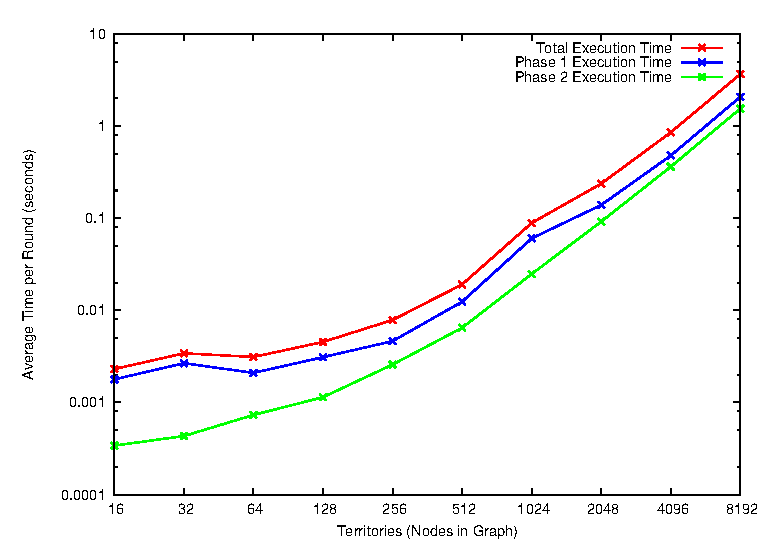
\includegraphics[width=.45\textwidth]{graphs.eps}
			%\vspace*{-10pt}
			\small{Figure 1: Performance of the algorithm on varying input sizes}
		\end{center}

		Utilizing 16 compute nodes, we ran the simulation on complete graphs with size $2^{n}$, with $n$ ranging from 4 to 13 (16 to 8192 vertices). 
		We noted that the computation time for complete graphs scaled exponentially with the number of vertices in the graph, which is entirely in keeping with our expectations. 
		Since the amount of work that must be done by the algorithm varies linearly with the number of edges in the graph, it varies exponentially with the number of vertices in the graph (going as $2^{vertices}$). 
		We notice in the graph that although phase 2 performs substantially less computation, it only runs slightly faster than phase 1. 
		This leads us to believe that the algorithm is largely dominated by its communication overhead. 
		The actual computation done during this algorithm is quite small compared to the sizeable round-robin sends - a near gigabyte of data movement (for a 8192 vertex graph) will naturally dominate a random conflict resolution function.
		We also note that the phase 1 curve is noticeably more irregular than the phase 2 curve, although its irregularity seems to smooth as the graph size increases. 
		This is due to the fact that we distribute computations on a per-territory basis, with a 50 percent chance that either territory involved in a conflict has its owner compute node handle the conflict. 
		The implication here is that slight load imbalances are likely responsible for the noise with small graph sizes, with the noise being reduced as graph size increases because the irregularities are amortized over a much larger sample space.
		The second scaling study we ran was a strong scaling study, with a various quantities of compute nodes working on a graph of 10080 vertices (we chose this number due to the fact that its evenly divisible by a large quantity of integers less than 16). 
		\begin{center}
			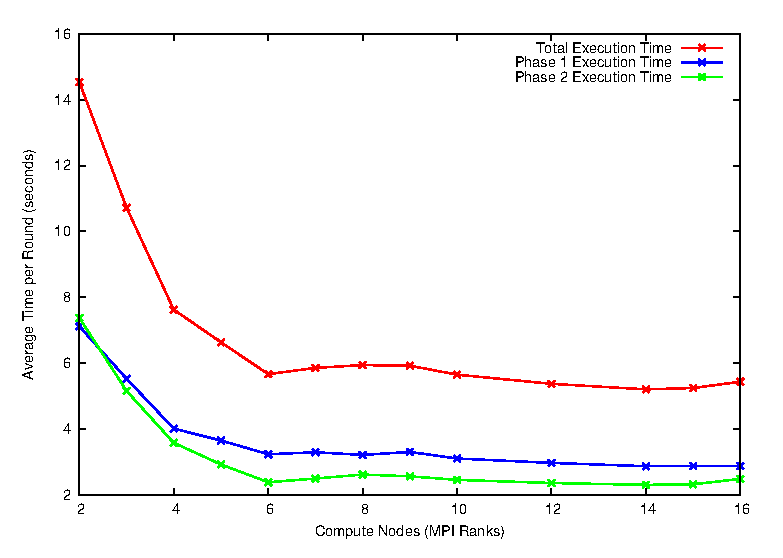
\includegraphics[width=.45\textwidth]{ranks.eps}
			%\vspace*{-10pt}
			\small{Figure 2: Strong scaling study (10080 vertex complete graph)}
		\end{center}
		
		We immediately notice that there seems to be a point of diminishing returns for a graph of this size. 
		Using greater than 6 compute nodes on an input of 8192 vertices seems to have a non-appreciable effect on the execution time of the algorithm. The reason for this immediate drop-off after a previously nearly direct correlation between more processors and speedup (from 2 to 6 compute nodes) is unclear, but it would appear that the sheer amount of data being passed around during the round robin phases is enough to counterbalance the speedup from doing less computational work per node. It is also possible that the (ever varying) load on the kratos server is responsible for slight inaccuracies with the data, but the other tests we ran seemed to verify these results.
				
		\section*{Conclusion}
		Our parallel turn-based conflict simulator was largely a success; it is able to provide "realistic" output given that the game it was created to model is largely based on chance.  
		Given that the simulation was difficult to parallelize due to its high degree of communication among territories in the graph, we observed an approximately linear speedup (3 compute nodes $\approx$ 1.5x speedup on an 8192-node complete graph) with an added number of compute nodes until 6 compute nodes was reached, at which point the simulation exhibited a plateau in performance (most likely indicating that the communication required was no longer benefitted by adding additional compute nodes).

		

		\section*{Related Work}
		Graph partitioning is a well-studied problem.  
		Our simulator used a trivial graph partitioning algorithm to divide up nodes among compute nodes.  
		Karypis and Kumar (IEEE HPC 1998) describe a parallel graph paritioning algorithm that promises high-performance partitioning with constraints on the partitioning schemes used.  
		In addition to graph partitioning, the distribution of computation among compute cores can be reduced to a variant of the NP-Complete edge-coloring problem as described by Holyer (Society for Industrial and Applied Mathematics, 1981); approximation algorithms exist to achieve a near-optimal solution (as described by Sanders and Steurer, ACM TALG, 2008).

		\section*{Future Work}

		Our successful results on Kratos lead us naturally to potentially explore further scaling studies at the massively parallel level; testing performance on the BlueGene/L system (and eventually the BlueGene/Q) would greatly enhance our insight into how our simulation performed as a result of performance and communication constraints.  
		Further performance optimizations would take into account more advanced approximation algorithms both for graph partitioning (to keep as many conflict resolutions local to a compute node as possible) and for even distribution of battle resolution calculation.  
		As previously mentioned, a next logical step from reducing communication requirements is to eliminate the need to exchange all simulation data at the end of each turn of the simulation.  
		Our results from running test cases on different types of input graphs, while preliminary, showed interesting trends that we would have liked to have explored more fully.  
		Future work in this area would include scaling studies in which the type of graph (or degree of connectedness) was studied for its effect on simulator performance.
		While our simulation was able to generate graphical representations in PNG format of intermediate battle situations (using the \emph{GraphViz} program), developing a method to visualize larger-scale conflict graphs in the thousands of nodes would be incredibly useful as the scale of the input grows.  
		With growing input scale, we also look to improving the overall ease of use of our simulator; while many of its features are already fairly modular, using a system such as a subclassed C++ implementation that enabled users to supply a strategy class would encourage interaction with the simulator and would facilitate better results. 

	\end{multicols}
\end{document}


%George Karypis and Vipin Kumar. 1998. Multilevel algorithms for multi-constraint graph partitioning. In Proceedings of the 1998 ACM/IEEE conference on Supercomputing (CDROM) (Supercomputing '98). IEEE Computer Society, Washington, DC, USA, 1-13.

